\begin{figure}[h!]
\begin{center}

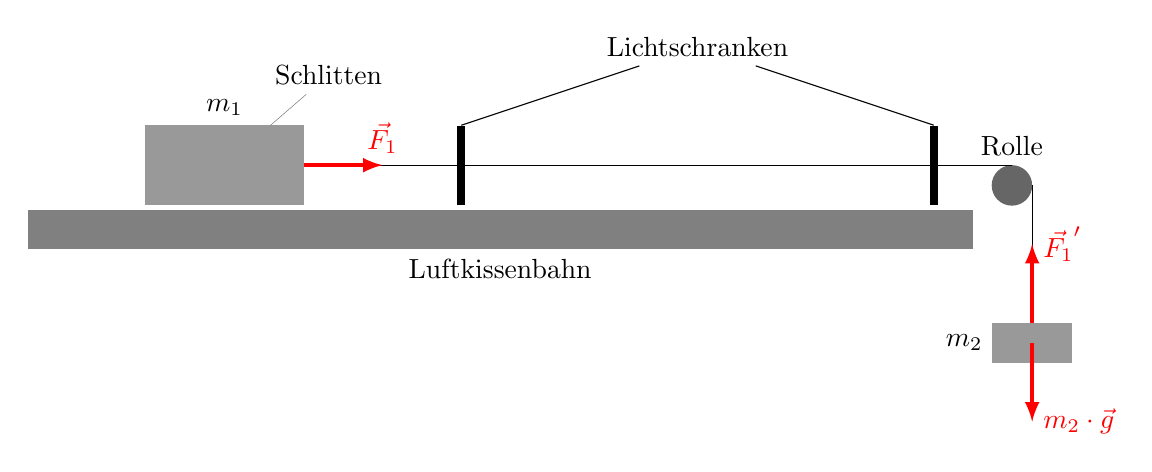
\begin{tikzpicture}
%\begin{tikzpicture}
%\usetikzlibrary{calc,intersections,through,backgrounds}
%\usetikzlibrary{decorations.pathmorphing}
%\draw[step=0.5cm,lightgray] (-0.5,-3.0) grid (6.5,5.0);
\usepgflibrary{arrows}
\tikzset{force/.style={>=latex,line width=0.05cm}}
%\newcommand{\RI}[2]{\ensuremath{#1_{\textrm{#2}}}}

\draw (5,0) node [minimum height=0.5cm, minimum width=12cm, fill, color=black!50,label=below:Luftkissenbahn] (B) {}; %bahn

\draw (B.north)+(-3.5cm,0.05cm) node [anchor=south,minimum height=1cm, minimum width=2cm,draw,fill, color=black!40, label=above:$m_1$,pin= 60:Schlitten] (M1) {}; %wagen

\draw (M1) +(10cm,0) node[anchor=north,circle,minimum size=0.5cm,draw,fill, color=black!60, label=above:Rolle] (R) {}; %rolle

\draw (R.east)+(0,-2cm) node[minimum height=0.5cm,minimum width=1cm,draw,label=left:$m_2$,fill,color=black!40] (M2) {}; %angehängtes gewicht

%\draw (M2.south)+(0,-1.2cm) node[minimum width=2cm, minimum height=0.1cm,anchor=north,fill,color=black!60, label=below:Tisch] (T){}; %Tisch

\draw (M1.east)--(R.north) (R.east)--(M2.north); %faden

%Kräfte
\draw [->,color=red,force] (M2.center)--+(-90:1cm) node [right] {$m_2\cdot \vec{g}$};
\draw[->,color=red,force] (M2.north)--+(90:1cm) node [right] {$\vec{F_1}'$};
\draw[->,color=red,force] (M1.east)--+(0:1cm) node [above]{$\vec{F_1}$};

 %Lichtschranke1}
\draw (M1.east)+(2cm,0) node[inner sep=0,minimum width=0.1cm,minimum height=1cm,fill] (L1){}; %Lichtschranke1

\draw (L1)+(6cm,0) node[inner sep=0,minimum width=0.1cm,minimum height=1cm,fill] (L2){}; %Lichtschranke1

\draw (L1.north)+(3cm,1.0cm) node (LL) {Lichtschranken};
\draw (LL)--(L1.north);
\draw (LL)--(L2.north);

\end{tikzpicture}

\end{center}
\caption{\label{fig:luftkissen} Ein Schlitten der Masse $m_1$ wird reibungsfrei auf einer Luftkissenbahn beschleunigt. 
Die Kraft $F_1$ entsteht durch die Gewichtskraft der Masse $m_2$, deren Richtung an einer Rolle umgelenkt wird.}
\end{figure}
\begin{aufgabe}
	Auf einer Luftkissenbahn steht ein Schlitten mit einer Masse von \SI{5}{kg} ($m_1$). Über eine Schnur ist $m_1$ mit einer anderen Masse
	von \SI{2}{kg} verbunden(siehe Abbildung \ref{fig:luftkissen}).
	Durch die Luftkissenbahn kann Reibung vernachlässigt werden.
	Wie gross ist die Beschleunigung?
	\begin{loesung}
		Die beschleunigende Kraft ist $F=m_2\cdot g$ die zu beschleunigende Masse ist $(m_1 +m_2)$.
		\begin{align*}
			F&=m\cdot a\\
			m_2\cdot g &= (m_1+m_2)\cdot a \to a=g\cdot\frac{m_2}{m1+m_2}=\SI{9.81}\cdot\frac{\SI{2}{kg}}{\SI{5}{kg}+\SI{2}{kg}}=\SI{2.8}{m/s^2}
		\end{align*}
	\end{loesung}
	\kloesung{$a=\SI{2.8}{m/s^2}$}
\end{aufgabe}



